\chapter{Proposed system}
\label{sec:proposed system}

\section{Overview}
A distributed system where a user is able to search and find movies. Information for the selected movie is displayed. He is able to add the found movie to his favourites list.

\section{Functional requirements}
\begin{itemize}
	\setlength{\itemsep}{-5pt}
	\item The following components shall be implemented
	\begin{itemize}
		\setlength{\itemsep}{-5pt}
		\item A database
		\item A server exposing functions for retrieving data from the database
		\item A Windows Application
		\item A web Client
	\end{itemize}
	\item All above parts shall be implemented in C\#. The Windows client in WPF and the web client in ASP.NET
	\item Communication between clients and server shall happen in a RESTful manner sending JSON over HTTP
	\item The server must build on the HttpListener for HTTP communication
	\item The server should support two ways of retrieving data. One being from its memory cache and the other begin from the Database. If the requested data is in memory it will be retrieved from there instead of from the Database
	\item The desktop client shall support two ways of storing data. One being XML on the disk, and another being in memory cache.
	\begin{itemize}
			\setlength{\itemsep}{-5pt}
			\item If the client is offline: If the requested data is in memory cache it will be retrieved from there instead of from the disk
			\item If the client is online: If the requested data is in memory cache it will be retrieved from there instead of from the disk. In both cases the client will check-up with the Server to see if it has the most recent version
	\end{itemize}
	\item The server shall be able to merge information from My Movie API. If some data is not stored locally, but is in the My Movie API, it will get the data from there and store it locally.
	\item The system shall allow for user registration and login
\end{itemize}

\section{Nonfunctional requirements}

\begin{itemize}

\item[\textbf{Usability}]
\begin{itemize}
\item A user with low PC expertise should be able to use the system
\end{itemize}

\vspace{0.2cm}
\item[\textbf{Reliability}]
\begin{itemize}
\item Reliability is a \textit{must} for the system. The user should experience as few software crashes as possible, with a maximum of 2 per day.
\item Restarting the system is acceptable if a software crash does happen
\item The system must not lose data as result of a software crash
\end{itemize}

\vspace{0.2cm}
\item[\textbf{Performance}]
\begin{itemize}
\item The system must be responsive even on the worst purchasable hardware today
\item The system should support at least 7 concurrent users
\item The server must support storing at least 10 gigabytes of data
\item The maximum latency the user can experience, when his internet is not a bottlenect, must not surpass 5 seconds
\end{itemize}

\vspace{0.2cm}
\item[\textbf{Supportability}]
\begin{itemize}
\item Extensibility
\begin{enumerate}
\item The system should be prepared for implementing more user functions
\item The system should be prepared for changing storage architecture
\end{enumerate}
\end{itemize}

\vspace{0.2cm}
\item[\textbf{Implementation}]
\begin{itemize}
\item The desktop client will be implemented for the Windows 7/8 operation system
\item The web client will be implemented by ASP.NET MVC
\end{itemize}

\vspace{0.2cm}
\item[\textbf{Interface}]
\begin{itemize}
\item The system shall interact with the My Movie API
\item Initial data for the movie database is made available as a .mdf file
\end{itemize}

\vspace{0.2cm}
\item[\textbf{Packaging}]
\begin{itemize}
\item The backend server software and database is installed by us
\item The Clients are installed by the end-user
\item The desktop client should be portable and not require any installation
\end{itemize}

\end{itemize}


\section{System models}

\subsection{Scenarios}
In order to specify the use cases in which the user can interact with the program, it is required to initially specify a couple of different scenarios the user can have while utilizing the application.

The following scenarios were set up in order to analyze them:

\begin{itemize}
	\setlength{\itemsep}{-5pt}
	
	\item John wants to find out the name of the actor playing the protagonist in Pulp Fiction. He searches for the title and information for the movie is retrieved.
	\item John liked the performance of Samuel L. Jackson in a movie, and wants to find other movies where he stars in. He searches for and selects Samuel L. Jackson, to enter his page, where a list of other movies is found.
	\item John wants to make a favourites list, but he needs a user account beforehand. He presses Register and enters his information. His user is now active.
	\item John has now made a user, and he wants to log in. He presses login and enters his login information.
	\item John loved Pulp Fiction, so he wants to add it to his favourites list. He searches and finds the movie, and presses the favourites icon in order to add it.
	
	\item The admin, George, has discovered that Will Smith is incorrectly called Woll Smoth, and needs to change the name back. He logs into his administrator account, and changes the name back.
	\item The new movie, The Hobbit 3, needs to be added to the database. The admin, George, logs into his administrator account. He notices that a new actor, Hans Lars Christiansen, is missing from the database. George adds both the actor and the movie to the database, and makes sure that the new actor is linked to the corresponding movie.
	\item George notices that he made a mistake when adding 'The Hobbit 3' to the database. He logs into his administrator account and edits the movie description accordingly.
	\item George realises that an incompetent intern has added a fake movie to the database. He promptly deletes it.
\end{itemize}

\subsection{Use case model}



\begin{itemize}
	\setlength{\itemsep}{-5pt}
	\item User
	\item Administrator
	\item Server
\end{itemize}

Through the inspection of the scenarios depicted in the Scenario’s section, we have deduced the use cases that the program should be able to support.

The use cases are as follows:

User use cases:
\begin{itemize}
	\setlength{\itemsep}{-5pt}
	\item Find movie
	\item Find actor
	\item Make account
	\item Add to favourites list
	\item Remove from favourites list
	\item View favourites list
	\item Log in to account
	\item Log out from account
\end{itemize}

Administrator use cases:
\begin{itemize}
	\item Add movie
	\item Edit movie information
	\item Delete movie
	\item Add actor
	\item Edit actor information
	\item Delete actor
\end{itemize}

After refining the system design, we have added the following boundary scenarios:
\begin{itemize}
	\setlength{\itemsep}{-5pt}
	
	\item Example
\end{itemize}

\begin{figure}[H]
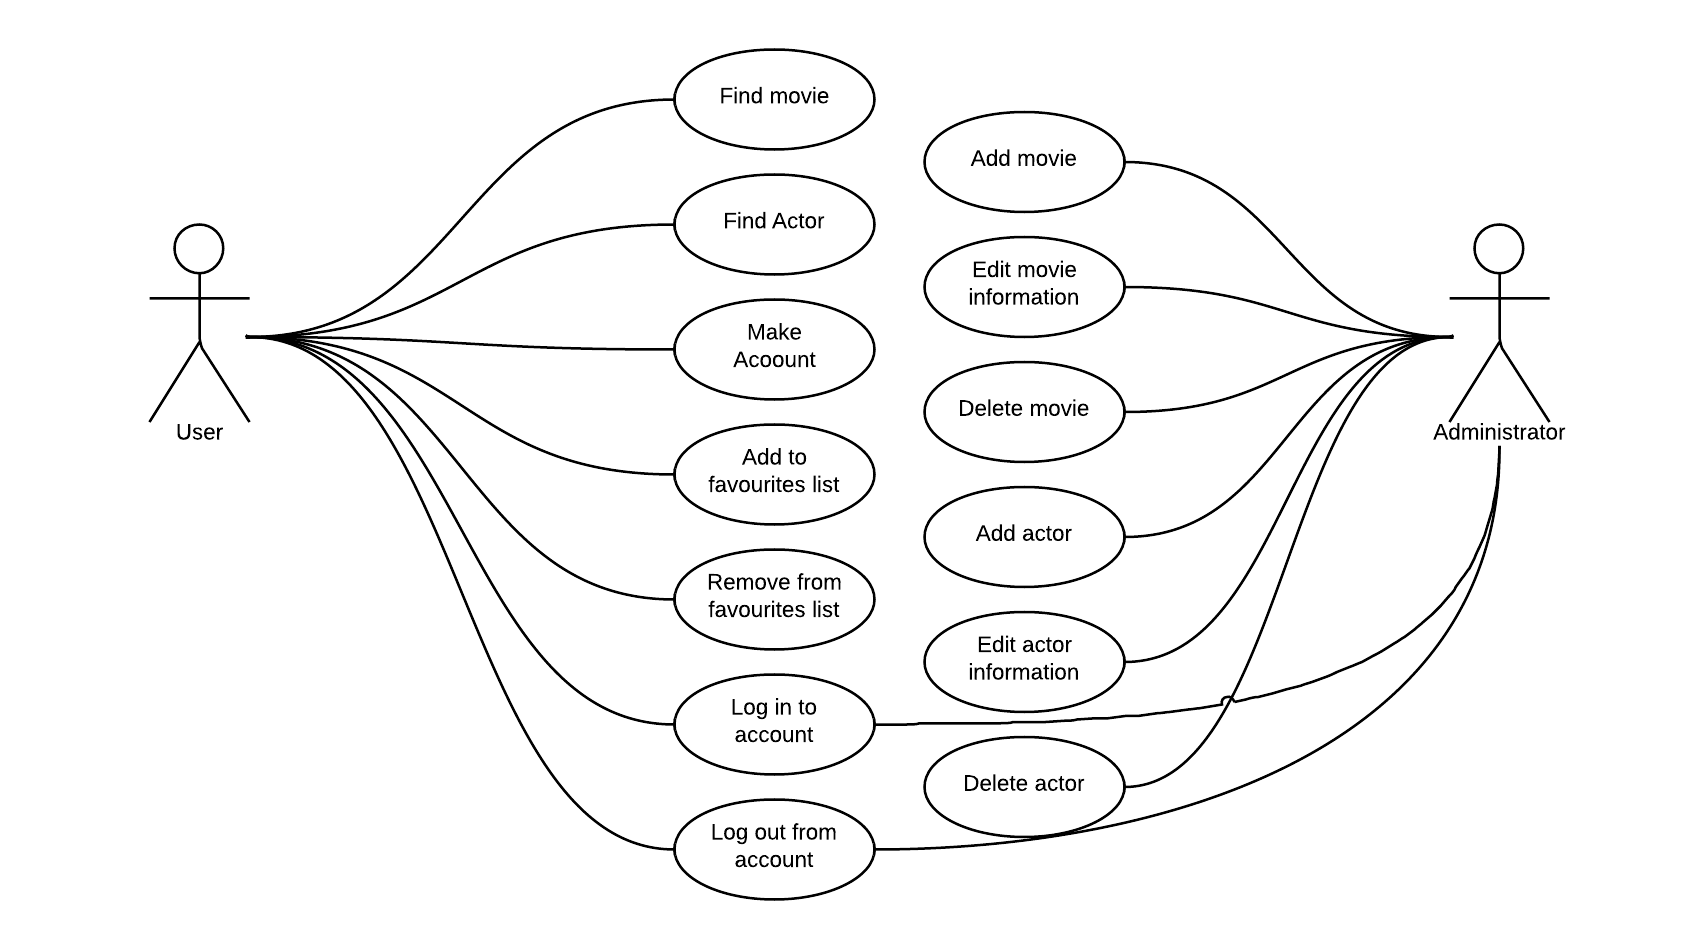
\includegraphics[width=\linewidth]{img/usecasediagram.png}
\caption{Use case diagram}
\label{fig:use case diagram}
\end{figure}

To have a more thorough understanding of each individual use cases, the following explanations was produced, describing each and every step of each use case.
The explanations furthermore include the relation between the actors and the use cases

\begin{center}
	\begin{tabular}{ | l | p{10cm} |  }
		 \hline
		Use Case Name & Find movie \\ \hline
		Participating Actors & Initiated by \emph{User} \\ \hline
		Flow of Events & \begin{enumerate}
						\item[1.] The \emph{user} searches for a movie
						\begin{enumerate}
							\item[2.] The client presents the user with a list of movies with names containing the input
						\end{enumerate}
						\item[3.] The \emph{user} selects one of the search results
						\begin{enumerate}
							\item[4.] The client displays a page containing information on the movie
						\end{enumerate}
					\end{enumerate} \\ \hline
		Entry Condition & \begin{itemize}
						\item The \emph{user} has a client open
					\end{itemize} \\ \hline
		Exit Condition & \begin{itemize}
						\item The \emph{user} successfully found a movie
					\end{itemize} \\
		\hline
	\end{tabular}
\end{center}


\subsection{Object model}

\subsubsection{Entity objects}

\begin{enumerate}
	\item[1.] Movie \hfill \\
	A movie is a collection of data about a specific movie. It has attributes defining its title, length, year of production and genre. Some movies are episodes of series and has attributes defining it's season and episode number.
	
	\item[2.] An People \hfill \\
	The people entity defines data about a specific person. Each entity instance includes attributes defining the name and the gender of the person. The person links to zero or more person information, describing further information such as age.
	
	\item[3.] User \hfill \\
	The user entity defines data about each specific user. Each entity instances includes attributes defining the log in informtion of the user. Each user has a list of favourite movies.
	
\end{enumerate}

\subsubsection{Boundary objects}

\begin{enumerate}

	\item[1.] Client \hfill \\
	The 'client', is a boundary object that allows the frontend program to contact the database. 

	\item[2.] Desktop Client \hfill \\
	The 'desktop client', is a specified version of the client, that is used in the desktop version of the application.
	
	\item[3.] Browser Client \hfill \\
	The 'browser client', is a specified version of the client, that is used in the browser version of the application.
	
\end{enumerate}

\subsubsection{Control objects}

These controllers are all more or less self-explanatory. They enable the user to realise all use cases from their client.

\begin{enumerate}
	\item[1.] FindMovieController
	\item[2.] FindActorController
	\item[3.] MakeAccountController 
	\item[4.] AddToFavouritesListController
	\item[5.] RemoveFromFavouritesListController
	\item[6.] ViewFavouritesListController
	\item[7.] LogInToAccountController
	\item[8.] LogOutFromAccountController 
	
	\item[9.] AddMovieController
 	\item[10.] EditMovieController
 	\item[11.] DeleteMovieController
 	\item[12.] AddActorController
 	\item[13.] EditActorController
 	\item[14.] DeleteActorController
 	
\end{enumerate}

\subsubsection{Class Diagram}

\begin{figure}[H]
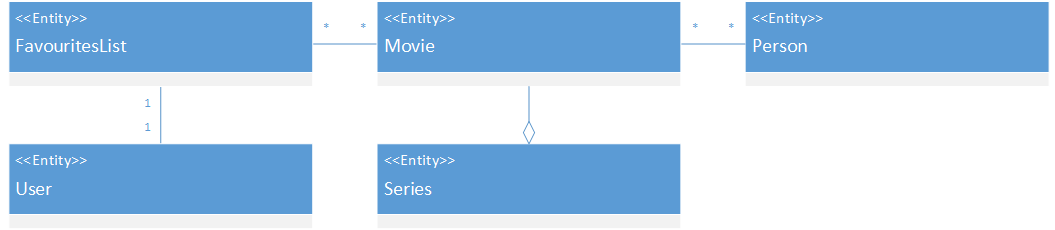
\includegraphics[width=\linewidth]{img/ClassDiagram.png}
\caption{Use case diagram}
\label{fig:use case diagram}
\end{figure}

\subsection{Dynamic model}



\subsubsection{Sequence diagrams}



\subsubsection{State machines}
An entity can have different states. As seen in figure \ref{fig:Entity State Machine Diagram}, after its creation (POST), it is stores in the persistent database module on the server. From here it can either be deleted (DELETE), or it can be fetched (GET). When a object is queried from the database the server will fetch it as a DTO (Data transfer object) into the servers memory. Often used objects will be saved in the server's cache. The DTO is then sent to the client requesting the object. The client-side also have a cache. This means that if the user has recently queried the object, it will not be fetched from the server, but from the local cache. A DTO can from there either be updated (PUT) and pushed back to the server, or cache time-out and be deleted (This means that only the DTO will be deleted and not the entity in the database).

This is valid for Movies and Actors. Users is not implementing these states as users should not be cached, and only have one state, which is In Database.   

\begin{figure}[H]
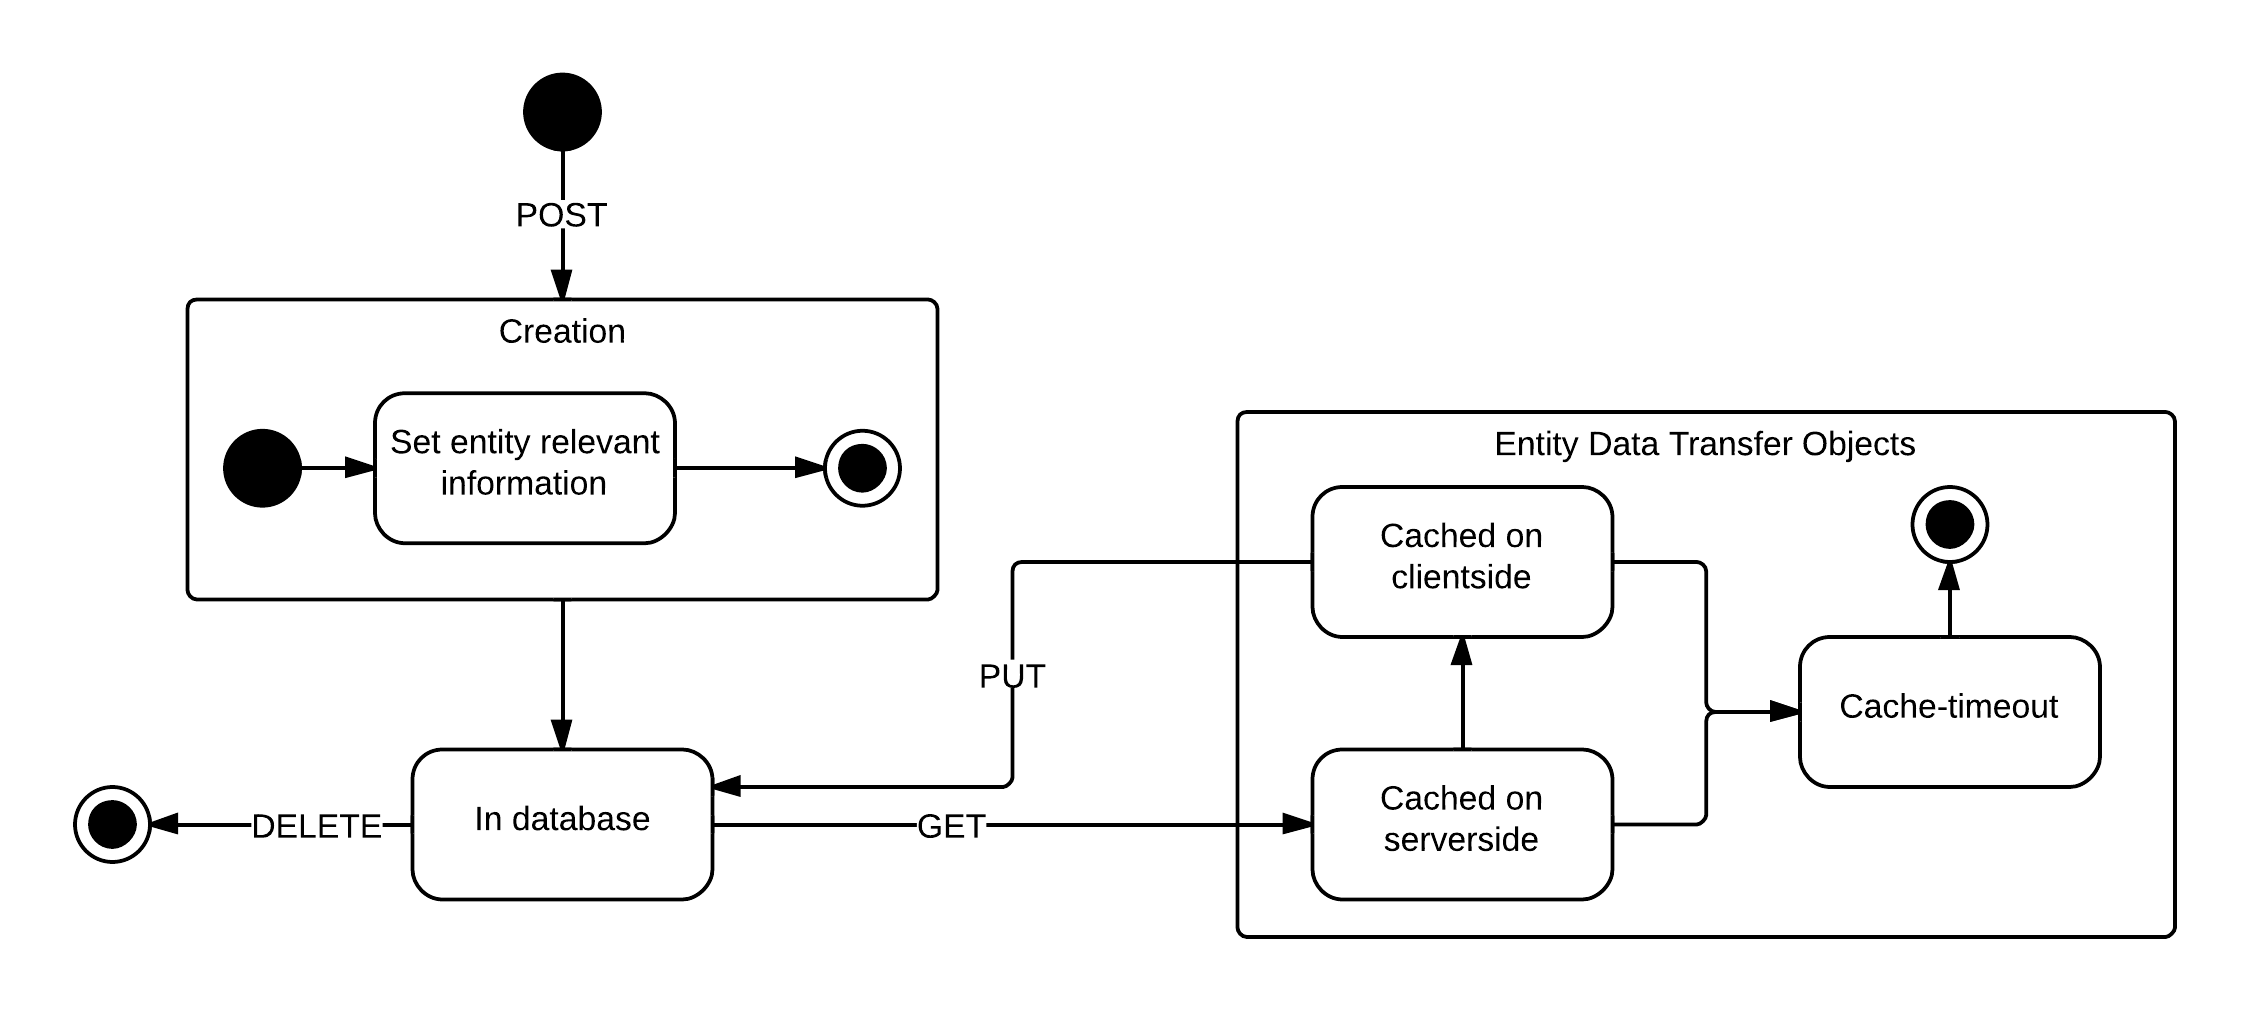
\includegraphics[width=\linewidth]{img/EntityStateMachineDiagram.png}
\caption{Entity State Machine Diagram}
\label{fig:Entity State Machine Diagram}
\end{figure}
\newpage
